


\begin{figure*}
  \begin{subfigure}[b]{0.49\textwidth}
    \centering
    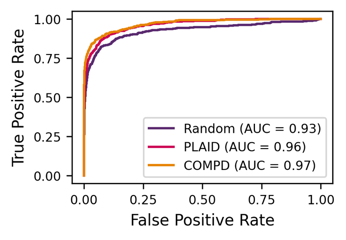
\includegraphics[width=\textwidth]{figures/ROC-10-10-0.2-1.png}
    \caption{1\% hits}
    %\label{fig:plaid-control-layout-bowl}
  \end{subfigure}
  \hfill
  \begin{subfigure}[b]{0.49\textwidth}
    \centering
    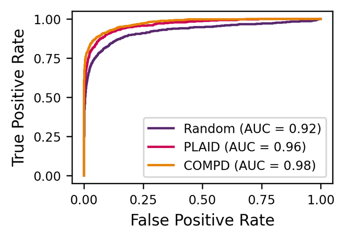
\includegraphics[width=\textwidth]{figures/ROC-10-10-0.2-5.png}
    \caption{5\% hits}
    %\label{fig:plaid-control-layout-bowl}
  \end{subfigure}

  
  \begin{subfigure}[b]{0.49\textwidth}
    \centering
    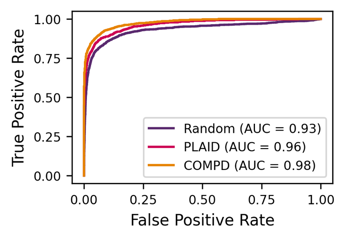
\includegraphics[width=\textwidth]{figures/ROC-10-10-0.2-10.png}
    \caption{10\% hits}
    %\label{fig:plaid-control-layout-bowl}
  \end{subfigure}
  \hfill
  \begin{subfigure}[b]{0.49\textwidth}
    \centering
    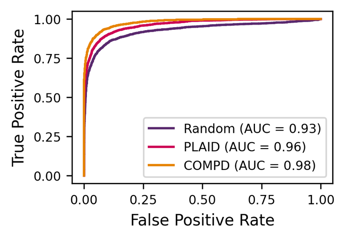
\includegraphics[width=\textwidth]{figures/ROC-10-10-0.2-20.png}
    \caption{20\% hits}
    %\label{fig:plaid-control-layout-bowl}
  \end{subfigure}

  \begin{subfigure}[b]{0.49\textwidth}
    \centering
    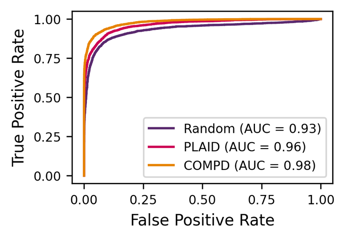
\includegraphics[width=\textwidth]{figures/ROC-10-10-0.2-30.png}
    \caption{30\% hits}
    %\label{fig:plaid-control-layout-bowl}
  \end{subfigure}
  \hfill
  \begin{subfigure}[b]{0.49\textwidth}
    \centering
    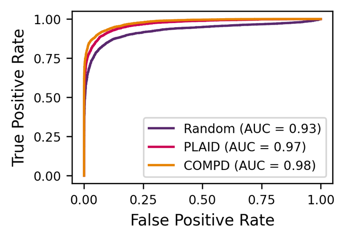
\includegraphics[width=\textwidth]{figures/ROC-10-10-0.2-40.png}
    \caption{40\% hits}
    %\label{fig:plaid-control-layout-bowl}
  \end{subfigure}
  
  \caption{Comparison of ROC curves for screening experiments with
    different hit rates, using layouts with 10 positive and 10
    negative controls in the presence of strong bowl-shaped plate
    effects.}
    \label{fig:screening-roc-10-10}
\end{figure*}




%%% Local Variables: 
%%% mode: latex
%%% TeX-master: "../supplement.tex"
%%% End: 
